% Use the `standard` option to get 4x3 aspect ratio.
% Use the `noul` option if there is a conflict with the `\ul` command.
\documentclass{antclass}
\newif\ifshow\showtrue

%\newcommand{\bf}{\mathbf}

%\pretitle{Version 2.2}
\title{Boltzmann Machine}
\subtitle{Overview and Prospects}
\author{Hooman Zolfaghari \\ Ramtin Moslemi \\ Borna Khodabandeh \\ Houman Jafari}

\begin{document}
\maketitle
\chapter{Machine Learning \& Physics}

\section{How are they related}
\begin{itemize}
	\item Bridge between physics and machine learning:
	\textbf{information}
	\item Amount of information = Extent of surprise
	\item Amount of information of event \( A = - \log \mathbb{P}(\text{event }A) \).

	\[
	\text{Little ``information''} \quad \Leftrightarrow \quad \text{difficult to predict} \quad \Leftrightarrow \quad \text{large information entropy}
	\]
	\[
	\text{A lot of ``information''} \quad \Leftrightarrow \quad \text{easy to predict} \quad \Leftrightarrow \quad \text{small information entropy}
	\]
	
	
\end{itemize}

\section{Maxwell’s demon \& Drawing Decisions}

  \begin{figure}[ht]
	\centering
	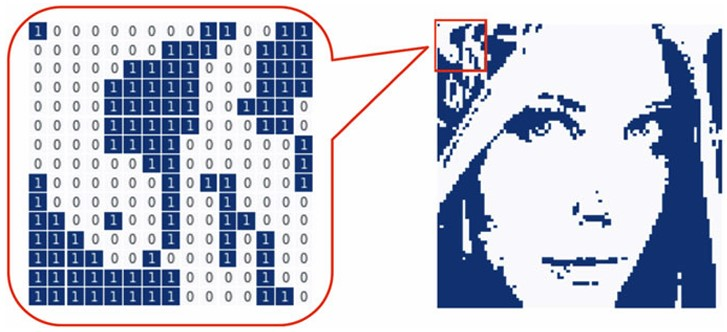
\includegraphics[width=0.8\linewidth]{pics/MLandPhysics/drawing.jpg}
%	\caption{}
	\label{fig:drawing}
\end{figure}



\section{Machine Learning Overview}
\begin{quote}
	 “\textit{Intelligence is not just about pattern recognition and function approximation. It’s about	modeling the world}”. — Josh Tenenbaum, NeurIPS 2021.
\end{quote}
	\begin{itemize}
		\item We have an observable space \(\mathcal{Z}\), a probability measure \(\mathbb{P}\), a sample \(S=\{Z_i\}_{i=1}^n\).
		\item Formulate the problem with a Hypothesis set \(\mathcal{H}\) and a "Loss function".
		\item (Ultimate goal) Statistical Risk: \(\arg\min_{h\in\mathcal{H}} R(h) = \mathbb{E}[\ell(h)]\)
		\item Empirical Risk: \(\hat{R}_S(h) = \frac{1}{n} \sum_{Z \in S} \ell(h(Z))  \)
	\end{itemize}
	
\section{Artificial Neural Network}

	\begin{itemize}
		\item A feed-forward neural network defines a function $f:\mathbb{R}^d\rightarrow \mathbb{R}^k$ recursively via layers .
		\[f(X) = f^{(L)}\circ f^{(L-1)}\circ \cdots \circ f^{(1)}(X) \quad f^{(i)}(X^{(i)})= \sigma(WX^{(i)}+b) \]
	\end{itemize}
	
	\textbf{Universal Approximation Theorem:}
	\begin{quote}
		\small For any continuous function $g:\mathbb{R}^d\rightarrow \mathbb{R}^k$ on a compact subset $K\subset \mathbb{R}^d$ and for any $\varepsilon>0$, there exists a neural network $f\in \mathcal{H}$ such that:
		\[
		\sup_{x\in K} \big|g(x)-f(x)\big| < \varepsilon.
		\]
	\end{quote}

\section{Training ANN}
\begin{itemize}
	
\item \textbf{Gradient Descent:}
\[
\theta\to f, \quad \theta_{t+1} = \theta_t - \eta \nabla_\theta \hat{R}_n(f)
\]


\item In infinite-width limit, the distribution over outputs of a randomly initialized neural network converges to a Gaussian Process%~\cite{neal1996priors}.
\item In gradient descent, the evolution of the network’s predictions can be approximated by a linear model characterized by the NTK:
\[
\Theta(x,x') = \langle \nabla_\theta f(x;\theta), \nabla_\theta f(x';\theta) \rangle.
\]
\item In infinite-width limit, the NTK can guarantee convergence under some assumptions.
\end{itemize}
 





\chapter{Energy Based Models}
\section{Outsource}

Outsourcing

\chapter{Boltzman Machine}
\section{Introduction}
\begin{itemize}
 	\item Idea was taken from statistical physics and formulated by cognitive scientists.
	
	\item The Hopfield network can reproduce specific patterns it has memorized
 	
 	\item Goal: "Understanding" the data instead of only memorizing
 	
 	\item Boltzmann machine can generate new patterns it has never seen before.
 	\item Multiple potential outputs (non-deterministic)
 	
 	\item "BM = Hopfield network + Stochasticity + Hidden Units"

 
\end{itemize}

\pagebreak

\begin{figure}[H]
		\centering
	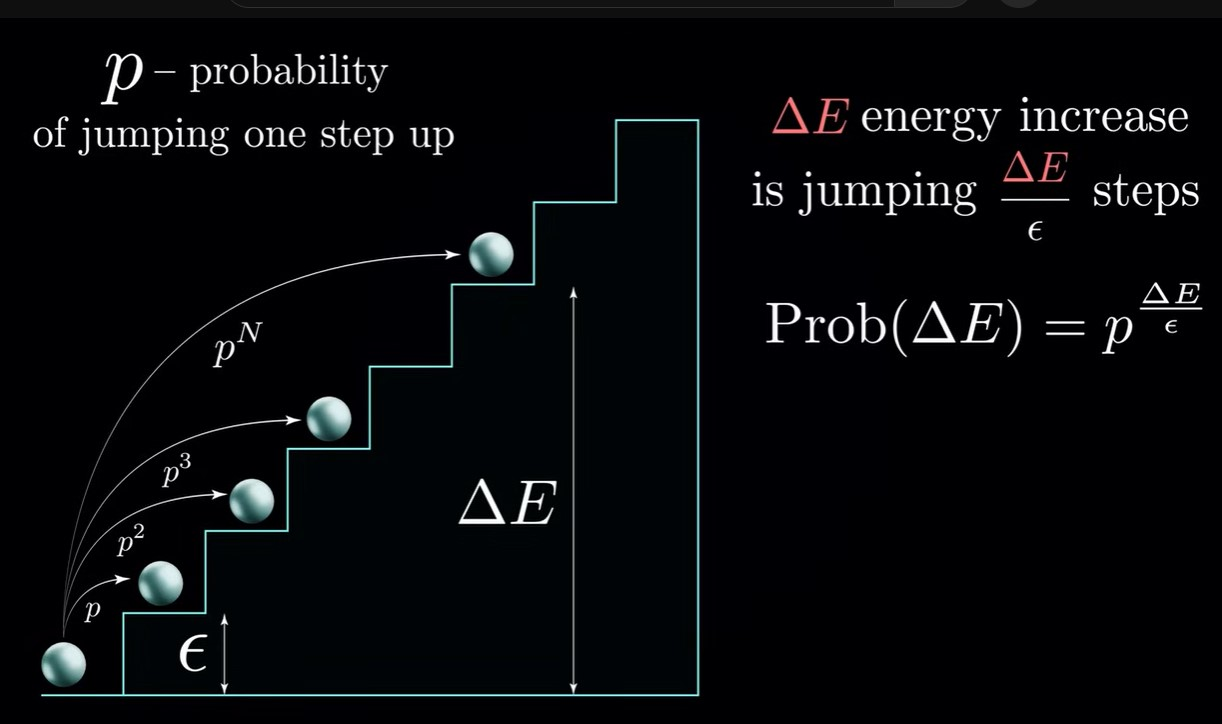
\includegraphics[width=0.8\linewidth]{pics/BM/Ball-Analogy.jpg}
	%	\caption{}
	\label{fig:ball-analogy}
\end{figure}

\pagebreak


\begin{itemize}
	\item We can formulate this by denoting \( T = \frac{-\ln(p)}{\epsilon}\), as:
	\begin{equation}
		\mathbb{P}(\Delta E) = e^{\frac{-\Delta E}{kT}}
	\end{equation}
	\item This gives us relative probability of changing energy.
	\item Knowing all probabilities have volume one, gives us absolute probability of each state.
	\item Giving us the partition function as the total volume.
	\begin{equation}
		\mathbb{P}(E) = \frac{1}{Z} e^{-E/T}
	\end{equation}
	
\end{itemize}


\section{Inference}
\begin{itemize}
	\item Hopfield Network's \textbf{deterministic} update rule:
	\[
	h_i = \sum_{j\neq i} w_{ij}x_j \rightarrow \text{input to neuron }i, \quad x_i = \begin{cases}
		+1 & h_i>0 \\ -1 & h_i <0
	\end{cases} \rightarrow \text{update rule}
	\]
	\item Always Greedy moving to the lowest energy state possible
	\item Boltzmann Machine update rule:
	\[
	 x_i = \begin{cases}
		+1 & \text{with probability }\mathbb{P}( E_{\text{on}}) \\
		-1 & \text{with probability }1-\mathbb{P}(E_{\text{off}})
	\end{cases}
	\]
\end{itemize}

\pagebreak

\begin{figure}[H]
			\centering
	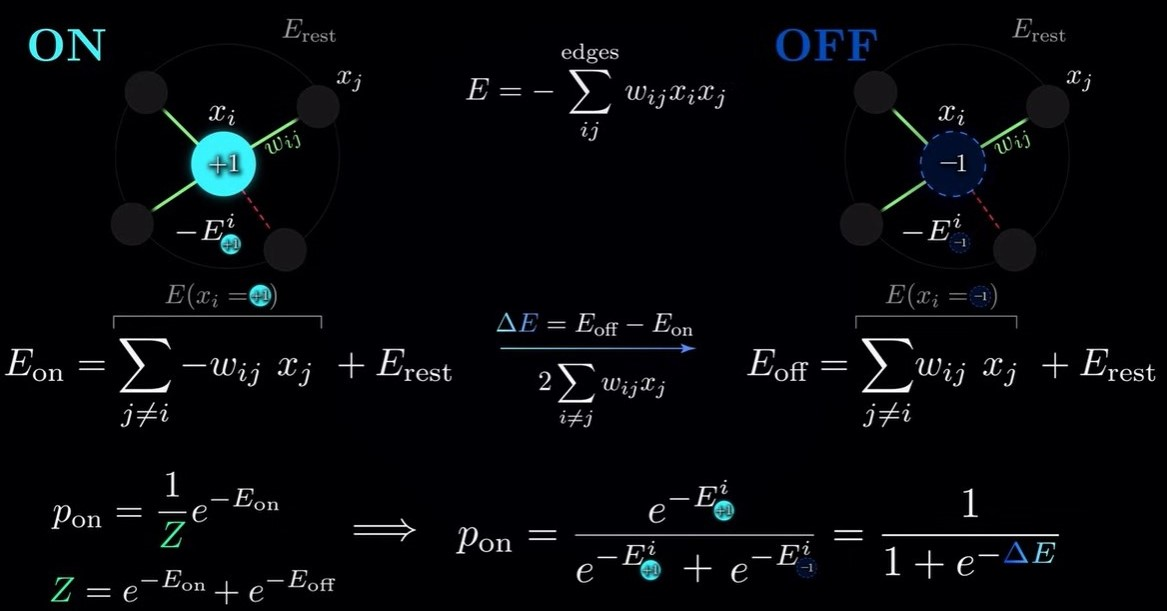
\includegraphics[width=\linewidth]{pics/BM/update-rule-hq.jpg}

	\label{fig:update-rule}
\end{figure}


\begin{figure}[H]
	\centering
	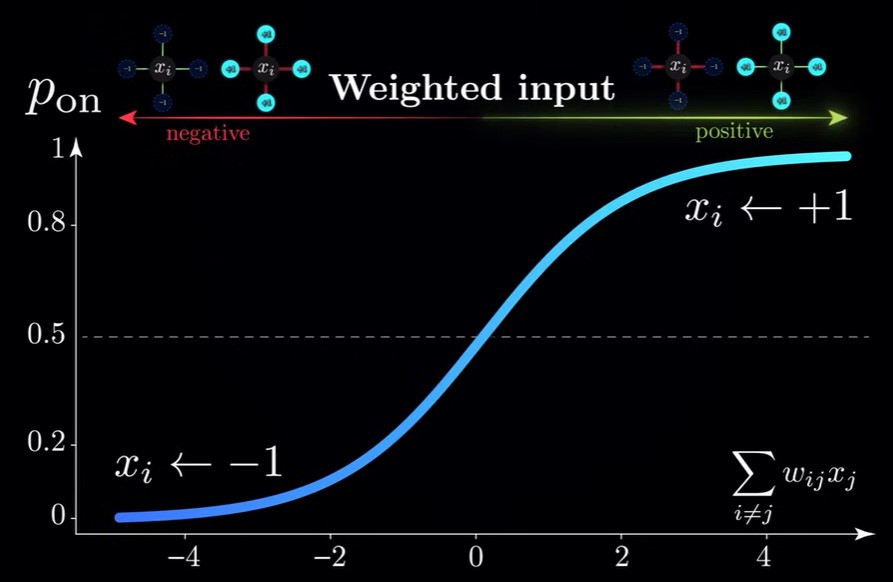
\includegraphics[width=0.8\linewidth]{pics/BM/sigmoid.jpg}
		\caption{Sigmoid activation \(\sigma(x)=\frac{1}{1+e^{-x}}\)}
	\label{fig:sigmoid}
\end{figure}

\begin{figure}[H]
	\centering
	\begin{minipage}[b]{0.5\linewidth}
		\centering
		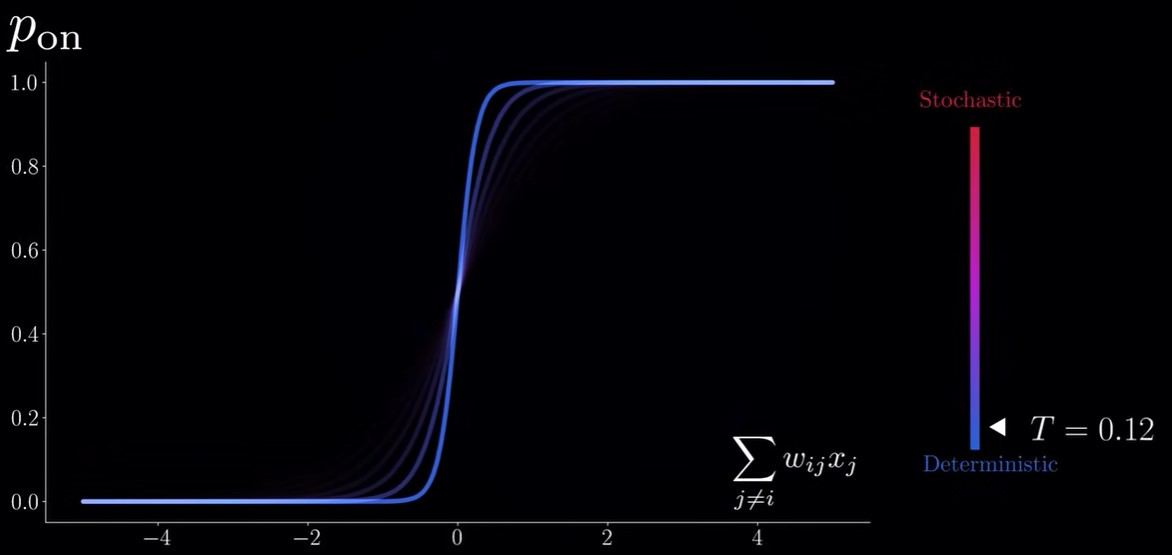
\includegraphics[width=\linewidth]{pics/BM/temp-low.jpg}

		\label{fig:temp-low}
	\end{minipage}
	
	\begin{minipage}[b]{0.5\linewidth}
		\centering
		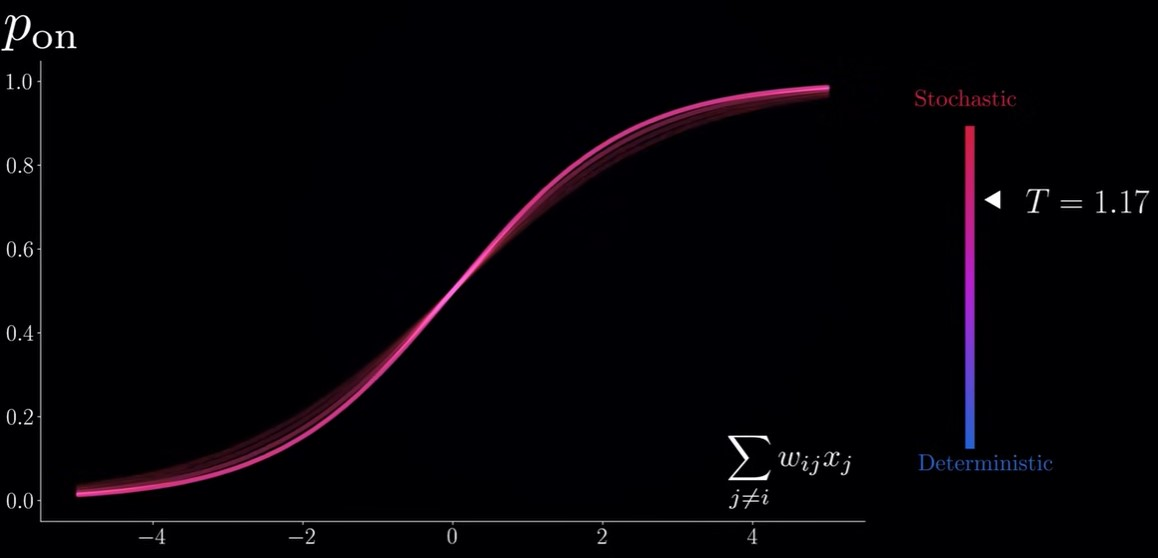
\includegraphics[width=\linewidth]{pics/BM/temp-high.jpg}
		
		\label{fig:temp-high}
	\end{minipage}
	
	\label{fig:both}
\end{figure}

\section{Learning}

\begin{itemize}
	\item Instead of memorizing patterns we want to learn probability distribution of data.
	\item We want the training data to have high probability
	\item Notice that increasing a states probability affects other states probability through partition function
	
		\[ \log \mathbb{P}(\text{data states}) = \sum_{i=1}^{N} \log(\frac{1}{Z} e^{-E(x^{(i)})/T}) \]
\end{itemize}
\pagebreak

\[
\underbrace{ \log \mathbb{P}(\text{data states}) }_{\text{Maximaize}} = -\frac{1}{T}[\sum_{i=1}^{N} \underbrace{E(x^{(i)})}_{\text{Minimize}} ]  - N \underbrace{ \log Z}_{\text{Minimize}}
\]

\begin{itemize}
\item Taking derivative with each \(w_{ij}\):
\begin{itemize}
	\item First term:( similar to Hopfield) \(\frac{\partial E(x^{(i)}) }{\partial w_{ij}} = -(x_ix_j)\)
	\item Second term: \(\frac{\partial \log Z}{\partial w_{ij}} = \sum_{s \in \text{all states}} \mathbb{P}(s)x_i^s x_j^s\)
\end{itemize}
\item Giving us the \textbf{Contrastive Hebbian Rule}:
\[
\Delta w_{ij} = \frac{1}{N} \sum_{n=1}^{N} x^{(n)}_ix^{(n)}_j - \mathbb{E}[ x_i^sx_j^s]
\]
\item second term computed by iterative sampling until equilibrium.
\end{itemize}


\section{Hidden Units}

\begin{figure}
	\centering
	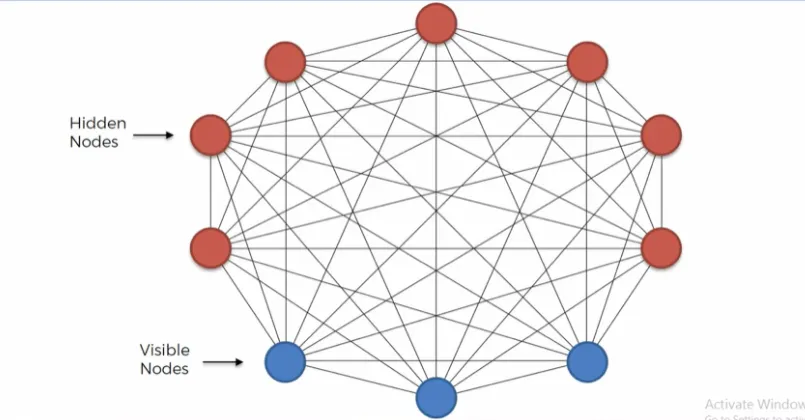
\includegraphics[width=0.8\linewidth]{pics/BM/BM.png}
	%	\caption{}
	\label{fig:bm-structure}
\end{figure}

\begin{itemize}

\item Visible Units: States directly encoding the data
\item Hidden Units: Internal representation of latent variables
\item We use the same update rule in inference
\item In Learning, input the data and sample the hidden state
\end{itemize}


\section{Energy Based Model}

\begin{itemize}
	 	
	\item Energy function:
	\[
	E(x;\theta) = - (\bf{x}^T\bf{Wx}+\bf{b}^T\bf{x})
	\]
	\item Parameters same as in \textit{Hopfield} networks and \textit{Ising} models
	
	\item Problem: Hard to train (due to the partition function)
	\item Solution:
	\begin{itemize}
		\item Introducing latent variables
		\item  Restricting connections among observables.
	\end{itemize}

\end{itemize}

\section{Restricting BMs}
\begin{itemize}
	\item Consider: binary observable variables \(\bf{x}\in \{0,1\}^D \) and binary latent (hidden) variables \(\bf{z}\in \{0,1\}^M\)
	\item The relationships among variables
	specified through this \textit{energy function}:
	\begin{equation}
		E(\bf{x,z};\theta) = - \bf{x}^T\bf{Wz}-\bf{b}^T\bf{x} -\bf{c}^Tx
	\end{equation} 
	\item For this EF, the RBM is defined by the \textit{Gibbs} distribution:
	\begin{equation}
	p(\bf{x,z};\theta) = \frac{1}{Z_\theta}\exp(-E(\bf{x,z};\theta))
	\end{equation}
	
	
\end{itemize} 

\pagebreak

\begin{itemize}
	\item the \textit{partition function}:
	\begin{equation}
		Z_\theta = \sum_{\mathbf{x}} \sum_{\mathbf{z}} \exp \big(-E(\mathbf{x}, \mathbf{z}; \theta)\big)
	\end{equation}
	\item The marginal probability over observables (the likelihood of observation):
	\begin{equation}
		p(\mathbf{x}|\theta) = \frac{1}{Z_\theta} \exp \big(-F(\mathbf{x}; \theta)\big)
	\end{equation}
	\item where \(F(\cdot)\) is the \emph{free energy}:
	\begin{equation}
		F(\mathbf{x}; \theta) = -\mathbf{b}^\top \mathbf{x} - \sum_j \log \big(1 + \exp(c_j + (\mathbf{W}_{\cdot j})^\top \mathbf{x}) \big).
	\end{equation}
\end{itemize}

\section{RBM}
\begin{itemize}
	\item The presented model is called a restricted Boltzmann machine (RBM).
	\item  Useful property: the conditional distribution over the hidden variables factorizes given the observable variables and vice versa:
	
	\begin{align}
		p(z_m = 1 | \mathbf{x}, \theta) &= \mathrm{sigm}\big(c_m + (\mathbf{W}_{\cdot m})^\top \mathbf{x}\big),  \\
		p(x_d = 1 | \mathbf{z}, \theta) &= \mathrm{sigm}\big(b_d + \mathbf{W}_{d \cdot} \mathbf{z}\big). 
	\end{align}
	
\end{itemize}

\section{Learning RBMs}
\begin{itemize}
	\item For given data \(\mathcal{D}=\{\mathbf{x}_n\}_{n=1}^N\) \item Train an RBM using the maximum likelihood
	\begin{equation}
		\ell(\theta) = \frac{1}{N} \sum_{\mathbf{x}_n \in \mathcal{X}} \log p(\mathbf{x}_n \mid \theta)
	\end{equation}
	\item The gradient with respect to \(\theta\):
\begin{align}
	\nabla_\theta \ell(\theta) &= -\frac{1}{N} \sum_{n=1}^N \big( \nabla_\theta F(\mathbf{x}_n; \theta) - \sum_{\mathbf{\hat{x}}} p(\mathbf{\hat{x}}|\theta) \nabla_\theta F(\mathbf{\hat{x}}; \theta) \big)
\end{align}
	\item Cannot be computed analytically because the second term requires summing over all configurations of observables.

\end{itemize}
\pagebreak

\begin{itemize}
	\item One way to sidestep this: Stochastic approximation
	\item  Replacing the expectation under \( p(\mathbf{x}|\theta) \) by a sum over \( S \) samples \(\{\mathbf{\hat{x}}_1, \ldots, \mathbf{\hat{x}}_S\}\) drawn according to \( p(\mathbf{x}|\theta) \):
	\begin{align}
		\nabla_\theta \ell(\theta) &\approx -\frac{1}{N} \sum_{n=1}^N \nabla_\theta F(\mathbf{x}_n; \theta) - \frac{1}{S} \sum_{s=1}^S \nabla_\theta F(\mathbf{\hat{x}}_s; \theta).
	\end{align}
\end{itemize}

\pagebreak
\begin{itemize}
	\item A different approach: \emph{contrastive divergence}
	\item Approximates the expectation under \( p(\mathbf{x}|\theta) \) by a sum over samples \(\mathbf{\tilde{x}}_n\) drawn from a distribution obtained by applying \( K \) steps of the block Gibbs sampling procedure:
	\begin{align}
		\nabla_\theta \ell(\theta) &\approx -\frac{1}{N} \sum_{n=1}^N \big( \nabla_\theta F(\mathbf{x}_n; \theta) - \nabla_\theta F(\mathbf{\tilde{x}}_n; \theta) \big). 
	\end{align}
	 
\end{itemize}

%\pagebreak
%
%\begin{itemize}
%	\item \textbf{Step 1: Sample hidden units.}
%	\[
%	z_m^{(t+1)} \sim \mathrm{Bernoulli}(\mathrm{sigm}(c_m + \mathbf{W}_{\cdot m}^\top \mathbf{x}^{(t)})).
%	\]
%	\item \textbf{Step 2: Sample visible units.}
%	\[
%	x_d^{(t+1)} \sim \mathrm{Bernoulli}(\mathrm{sigm}(b_d + \mathbf{W}_{d \cdot} \mathbf{z}^{(t+1)})).
%	\]
%	
%	    \item \textbf{Positive Phase:} Compute \( \nabla_\theta F(\mathbf{x}_n; \theta) \) at data point \( \mathbf{x}_n \).
%	\item \textbf{Negative Phase:} Run Gibbs sampling for \( K \) steps to obtain \( \mathbf{\tilde{x}}_n \), then compute \( \nabla_\theta F(\mathbf{\tilde{x}}_n; \theta) \).
%	\item \textbf{Gradient Approximation:}
%	\[
%	\nabla_\theta \ell(\theta) \approx \frac{1}{N} \sum_{n=1}^N \big( \nabla_\theta F(\mathbf{x}_n; \theta) - \nabla_\theta F(\mathbf{\tilde{x}}_n; \theta) \big).
%	\]
%	
%\end{itemize}

\pagebreak

\begin{itemize}

	\item The original CD used K steps of the Gibbs chain, starting and is restarted after every parameter
	update.
	\item An alternative approach, Persistent Contrastive Divergence (PCD)
	does not restart the chain after each update
	typically resulting in a slower
	convergence rate but eventually better performance 
\end{itemize}

\section{Higher-Order Relationships }

\begin{itemize}
	\item The energy function allows the modeling of
	higher-order dependencies among variables.
	\item For instance: Third-order multiplicative interactions by introducing two kinds of hidden	variables
	\begin{itemize}
		\item \textbf{Subspace Units:} Reflect feature variations, robust to invariances:
		\item \textbf{Gate Units:} Activate subspace units, pool subspace features.
	\end{itemize}
\end{itemize}

\pagebreak
\subsection{Random Variables for SubspaceRBM}
\begin{itemize}
	\item Observables: \( \mathbf{x} \in \{0, 1\}^D \).
	\item Gate Units: \( \mathbf{h} \in \{0, 1\}^M \).
	\item Subspace Units: \( \mathbf{S} \in \{0, 1\}^{M \times K} \).
	\item \textbf{Connections:} \( x_i \), \( h_j \), and \( s_{jk} \).
\end{itemize}

\pagebreak

\subsection{Energy Function for SubspaceRBM}
	\begin{align}
	E(\mathbf{x}, \mathbf{h}, \mathbf{S}; \theta) =
	-\sum_{i=1}^D \sum_{j=1}^M \sum_{k=1}^K W_{ijk} x_i h_j s_{jk} \nonumber \\
	-\sum_{i=1}^D b_i x_i 
	-\sum_{j=1}^M c_j h_j 
	-\sum_{j=1}^M h_j \sum_{k=1}^K D_{jk} s_{jk},
	\end{align}
	\[
	\theta = \{W, \mathbf{b}, \mathbf{c}, \mathbf{D}\}, \quad 
	W \in \mathbb{R}^{D \times M \times K}, \quad \mathbf{b} \in \mathbb{R}^D, \quad \mathbf{c} \in \mathbb{R}^M, \quad \mathbf{D} \in \mathbb{R}^{M \times K}.
	\]
	
	
\pagebreak
\subsection{Conditional Distributions in SubspaceRBM}
\begin{gather}	
	p(x_i = 1 | \mathbf{h}, \mathbf{S}) = \mathrm{sigm}\left(\sum_j \sum_k W_{ijk} h_j s_{jk} + b_i\right) \\
	p(s_{jk} = 1 | \mathbf{x}, h_j) = \mathrm{sigm}\left(\sum_i W_{ijk} x_i h_j + h_j D_{jk}\right) \\
	p(h_j = 1 | \mathbf{x}) = \mathrm{sigm}\left(-K \log 2 + c_j + \sum_{k=1}^K \mathrm{softplus}\left(\sum_i W_{ijk} x_i + D_{jk}\right)\right)
\end{gather}

\chapter{Renormalization Group}
\section{Introduction to Renormalization Group (RG)}

\textbf{The Renormalization Group (RG)} is a mathematical framework used to study lengths or energy scales, particularly in statistical physics and quantum field theory.

\begin{equation}
e^{-H_{\text{RG}, \theta}[\{h_j\}]} \equiv \sum_{v_i}e^{T_\theta(\{v_i\}, \{h_j\}) - H(\{v_i\})}
\end{equation}

\begin{figure}
    \centering
    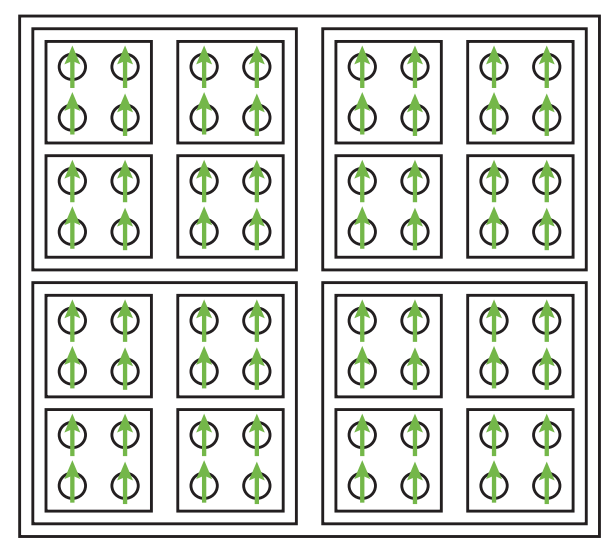
\includegraphics[width=0.55\linewidth]{pics/Renormalization/BlockSpin.png}
\end{figure}

\pagebreak

\section{RG in the 1D Ising Model}

The RG approach can be illustrated with the one-dimensional Ising model. Without a magnetic field, the partition function $Q$ is given by
($K = J / (k_B T)$):\begin{equation}
Z(K, N) = \sum_{s_1, s_2, \dots, s_N = \pm 1} \exp \big[ K(s_1s_2 + s_2s_3 + s_3s_4 + \dots) \big],
\end{equation}
\textbf{Decimation:} Summing over even-numbered spins reduces the problem size.
\begin{equation}
Z(K', N) = \sum_{s_1, s_3, \dots} \big[ \exp(K' s_1 s_3) + \exp(-K' s_1 s_3) \big] \cdots.
\end{equation}
\begin{figure}
    \centering
    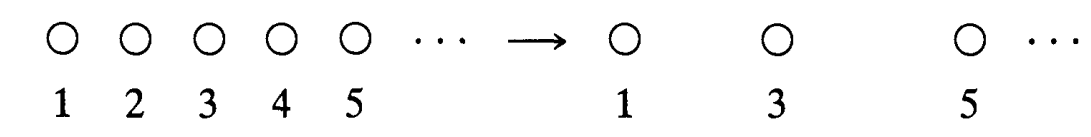
\includegraphics[width=0.90\linewidth]{pics/Renormalization/SumOverEven.png}
\end{figure}

\pagebreak

\section{Hidden Units in RBMs}

\textbf{Restricted Boltzmann Machines (RBMs)} consist of visible ($v$) and hidden ($h$) units:
\begin{equation}
P(v, h) = \frac{1}{Z} \exp \big( \sum_i a_i v_i + \sum_j b_j h_j + \sum_{i, j} v_i W_{ij} h_j \big).
\end{equation}
Hidden units simplify data by marginalizing over $h$:
\begin{equation}
P(v) = \sum_h P(v, h).
\end{equation}
RBM Hamiltonian for the hidden units:
\begin{equation}
p_\theta(\{h_j\}) \equiv \frac{e^{-H_{\text{RBM}, \theta}[\{h_j\}]}}{Z}.
\end{equation}
hidden units condition over visible units:
\begin{equation}
T(\{v_i\}, \{h_j\}) = -E(\{v_i\}, \{h_j\}) + H[\{v_i\}].
\end{equation}

\pagebreak

\section{Mapping RG to Hidden Units in RBMs}

We divide both sides of Eq. 18 by Z to get:
\begin{equation}
\frac{e^{-H_{\text{RG}, \theta}[\{h_j\}]}}{Z} = \frac{\sum_{v_i}e^{T_\theta(\{v_i\}, \{h_j\}) - H(\{v_i\})}}{Z}
\end{equation}
Substituting Eq. 24 into this equation yields
\begin{equation}
\frac{e^{-H_{\text{RG}, \theta}[\{h_j\}]}}{Z} = \frac{\sum_{v_i}e^{-E(\{v_i\}, \{h_j\})}}{Z} = p_\theta(\{h_j\})
\end{equation}
Substituting Eq. 23 into the right-hand side yields the
desired result
\begin{equation}
H_{\text{RG}, \theta}[\{h_j\}] = H_{\text{RBM}, \theta}[\{h_j\}]
\end{equation}
\textbf{Analogy:}
\begin{itemize}
\item RG reduces degrees of freedom (e.g., decimation of spins).
\item Hidden units in RBMs marginalize over latent variables.
\end{itemize}

\pagebreak

\section{Deep Architectures and RG}

\[
e^{T(\{v_i\}, \{h_j\})} = e^{-E(\{v_i\}, \{h_j\}) + H[\{v_i\}]}
\]

\[
= \frac{p_\theta(\{v_i\}, \{h_j\})}{p_\theta(\{v_i\})} e^{H[\{v_i\}] - H_{\text{RBM}, \theta}[\{v_i\}]}
\]

\[
= p_\theta(\{h_j\}|\{v_i\}) e^{H[\{v_i\}] - H_{\text{RBM}, \theta}[\{v_i\}]}
\]
only when RG satisfies
\[
\sum_{h_i}e^{T_\theta(\{v_i\}, \{h_j\})} = 1
\]
we can obtain
\[
H[\{v_i\}] = H_{\text{RBM}, \theta}[\{v_i\}]
\]

\pagebreak

\section{Summery}

\begin{figure}[h!]
    \centering
    \begin{minipage}{0.45\textwidth}
        \centering
        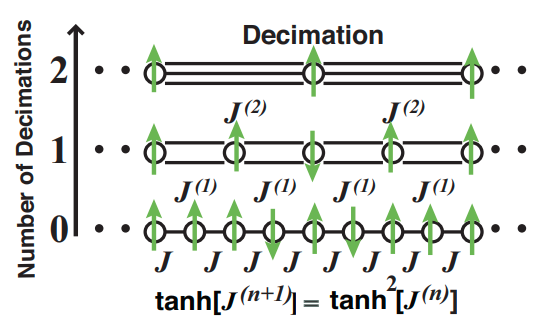
\includegraphics[width=\linewidth]{pics/Renormalization/Decimation.png}
    \end{minipage} \hfill
    \begin{minipage}{0.45\textwidth}
        \centering
        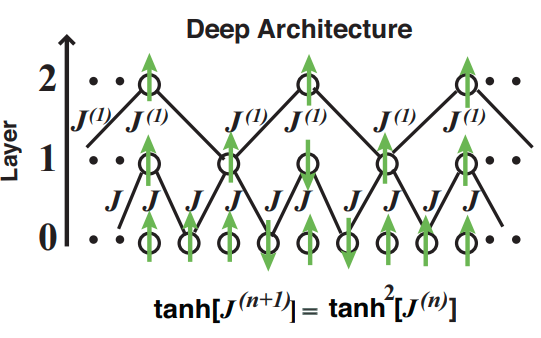
\includegraphics[width=\linewidth]{pics/Renormalization/DeepLayers.png}
    \end{minipage}
\end{figure}

Deep architectures in neural networks are analogous to RG transformations:
\begin{itemize}
\item Layers correspond to successive RG steps.
\item Hidden units represent coarse-grained variables.
\end{itemize}

\pagebreak

\chapter{Adversarial Examples}

\section{Adversarial Examples}
\begin{figure}
	\centering
	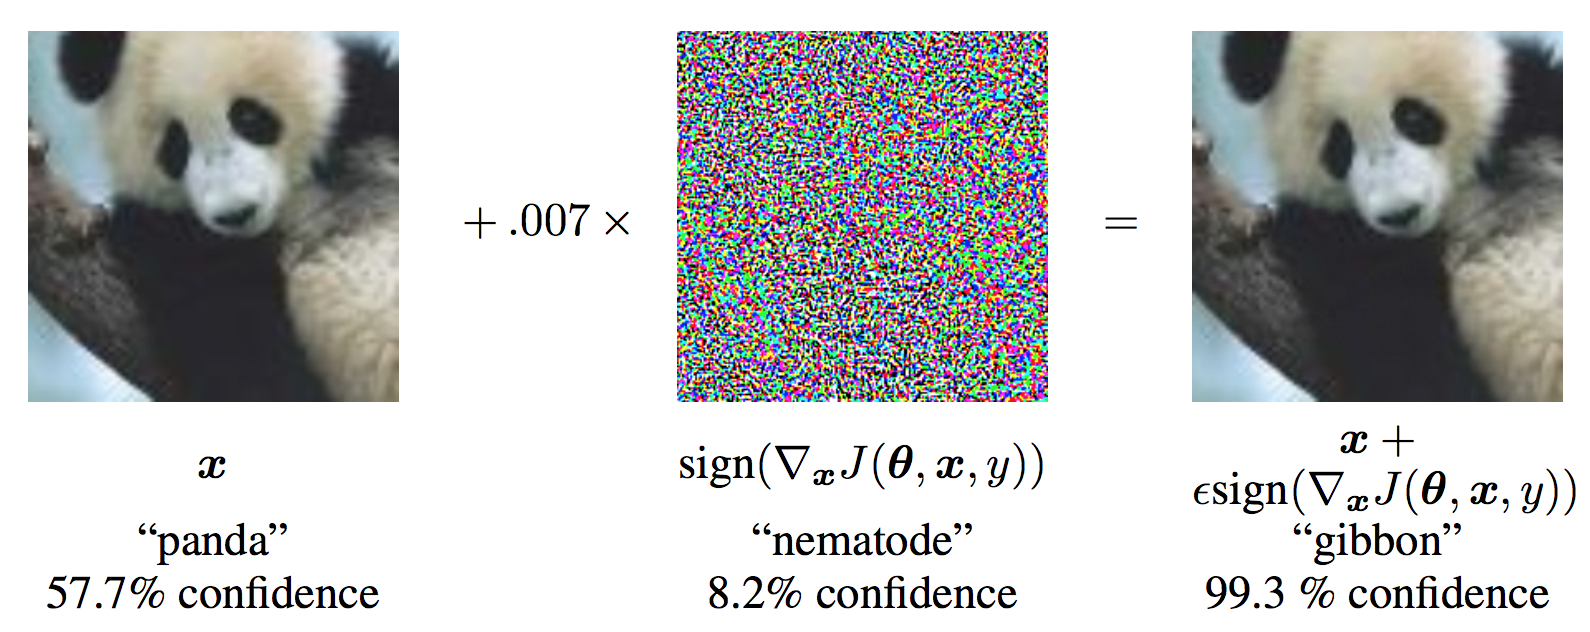
\includegraphics[width=0.8\linewidth]{pics/fgsm_panda_image.png}
	%	\caption{}
	\label{fig:panda}
\end{figure}

\section{Adversarial Examples}
\begin{itemize}
	\item We are to perturb all images such that they get misclassified.
	\item Both previously seen and unseen data are vulnerable.
	\item Defensive methods based on gradient obfuscation don't work.
	\item Over the years more advanced attacks have been introduced.
	\item The general idea is to generate adversarial examples using:
	$$x_{adv} = x + \delta , \quad \delta = \arg \max L(x+\delta , y), ~\|\delta \| \le \epsilon$$
\end{itemize}

\section{Adversarial Training}
\begin{itemize}
	\item While most other defenses fail, adversarial training works (kind of):
	$$
	\min_\theta \mathbb{E}_{(x,y)\in \mathcal{D}}\left[\max_{\delta \in \mathcal{S}} L(\theta, x+\delta, y)\right]
	$$
		\item In AT we are faced with a minmax optimization problem.
		\item Sadly, AT reduces clean accuracy and is very time consuming.
		\item More recent works address these issues.
\end{itemize}

\chapter{ Restricted Hopfield Networks are Robust to Adversarial Attack}
\section{Dense Associative Memory}
\begin{itemize}
	\item DAM was proposed to improve the storage limitation of the Hopfield Neural Network.
	\item DAM uses super-linear memory storage capacity as a function of the number of feature neurons.
	%\item Modern Hopfield Network (MHN) facilitate the storage and retrieval of raw input data, intermediate results, or learned prototypes.
	\item Using a gradient decent in the pixel space, a set of rubbish images is constructed that correspond to the minima of the objective function used in training.
	\item As the power of the interaction vertex is increased the images gradually become less speckled and more semantically meaningful.
\end{itemize}
\section{Image Generation}

\begin{figure}
	\centering
	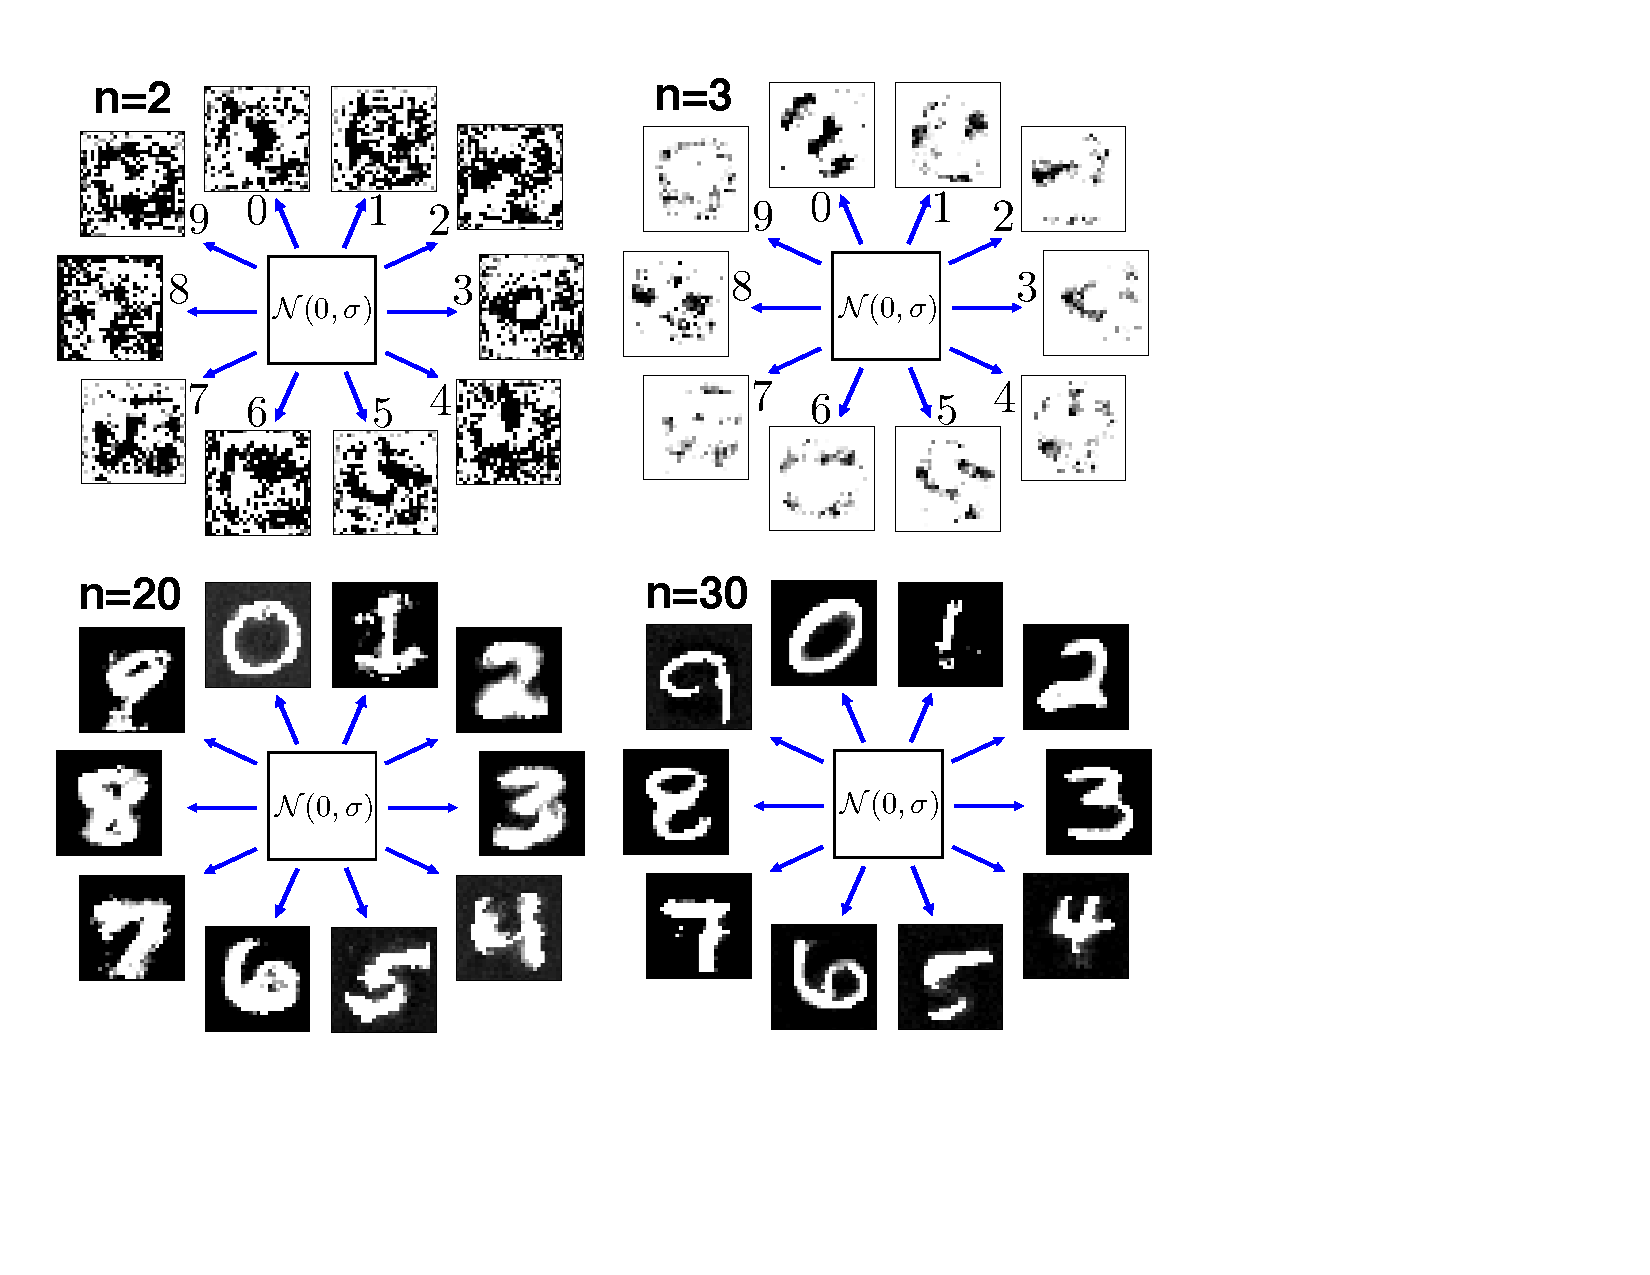
\includegraphics[width=0.55\linewidth]{pics/Rubbish_n_2_3_20_30}
\end{figure}

\section{Adversarial Examples}
\begin{figure}
	\centering
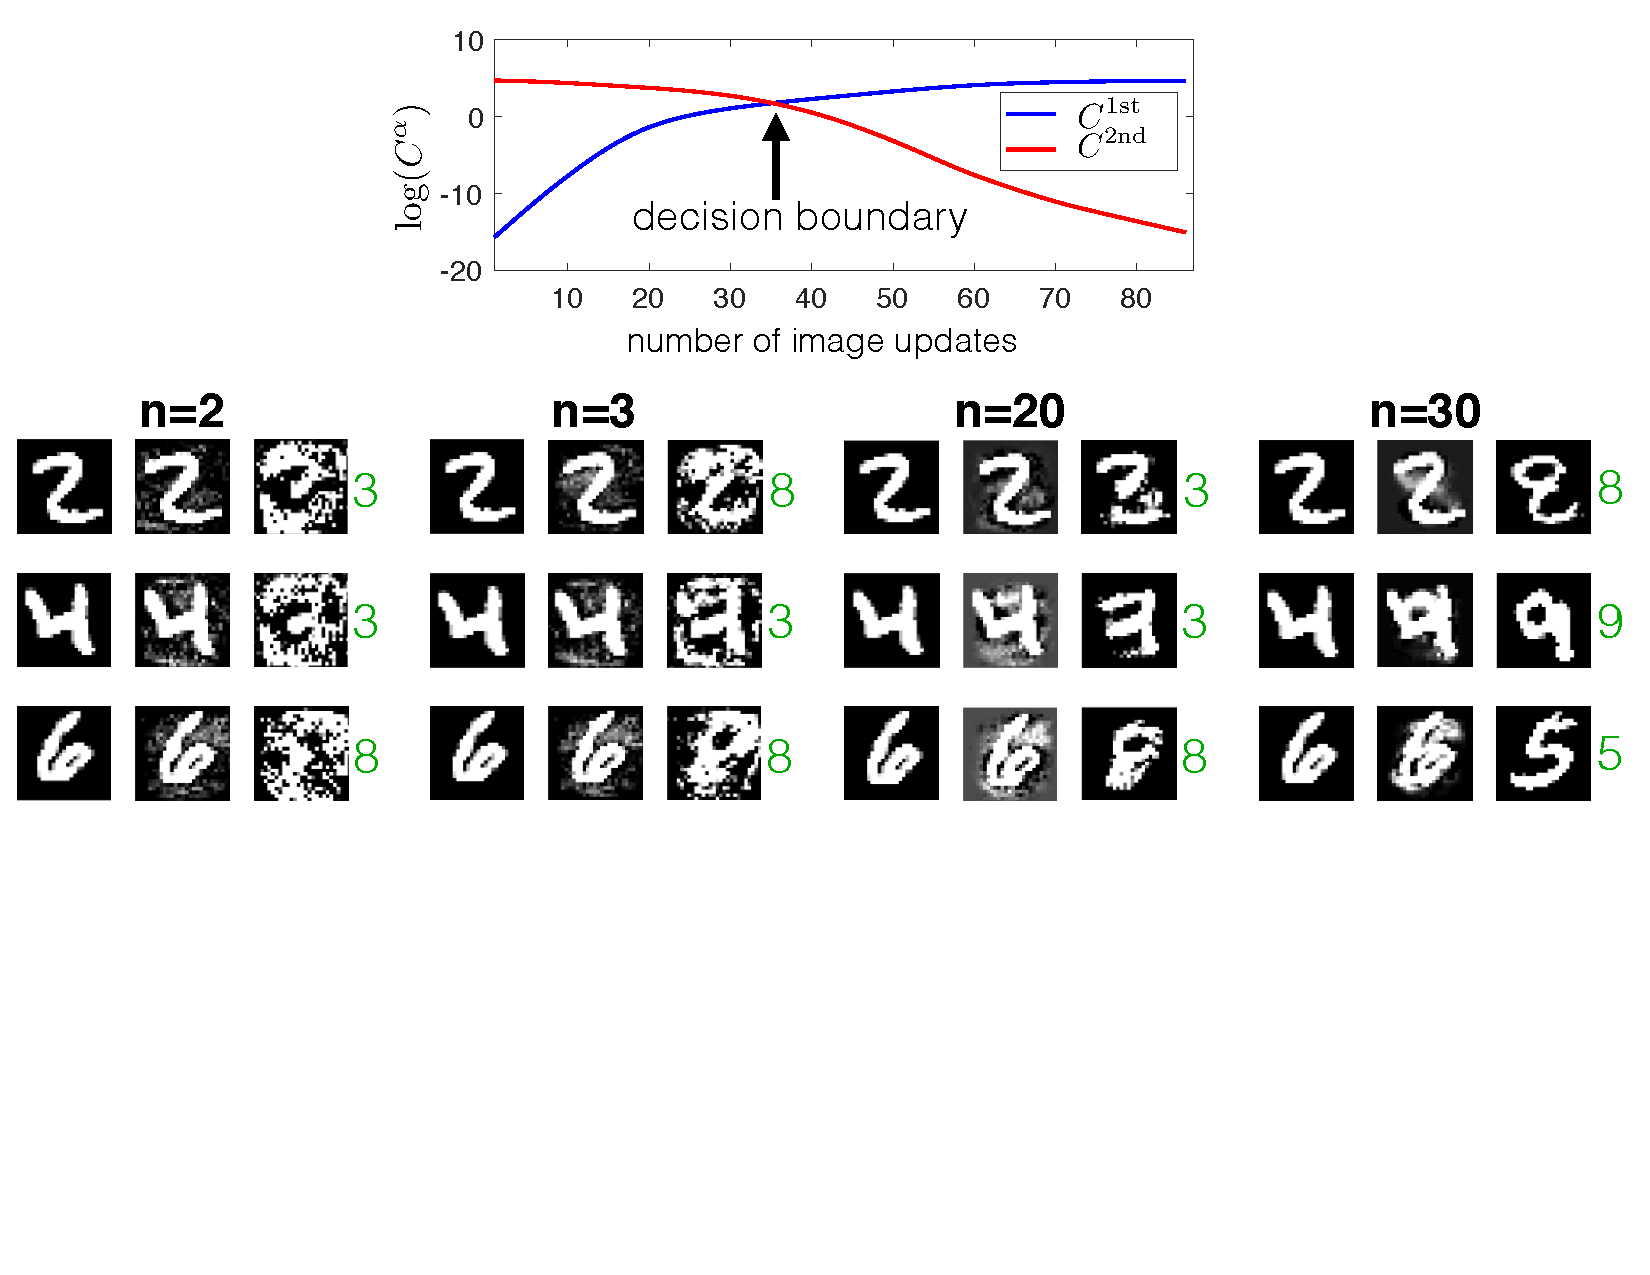
\includegraphics[width=\linewidth]{pics/Adv_deform}
\end{figure}

\closing
\end{document}
